\documentclass[12pt,a4paper]{article}
\usepackage[utf8]{vietnam}
\usepackage{amsmath,amssymb}
\usepackage{geometry}
\geometry{top=1.5cm,bottom=1.2cm,left=1.4cm,right=1.4cm,headheight=28pt,headsep=12pt,footskip=18pt}
\usepackage{tikz}
\usepackage{xcolor}
\usepackage{enumerate}
\usepackage{graphicx}
\usepackage[version=4]{mhchem}
\usepackage{fancyhdr}
\usepackage{ex_test}

\renewcommand{\baselinestretch}{0.96}
\setlength{\parskip}{0pt}

\definecolor{hfRed}{RGB}{211,47,47}
\definecolor{hfGreen}{RGB}{139,195,144}

\pagestyle{fancy}
\fancyhf{}
\fancyhead[L]{\small\itshape\color{hfRed} Tài liệu lưu hành nội bộ}
\fancyhead[R]{\small\itshape\color{hfRed} Thầy \textbf{TRẦN VĂN THẠNH} - 0777.470.803}
\renewcommand{\headrulewidth}{0.8pt}
\renewcommand{\headrule}{\hbox to\headwidth{\color{hfGreen}\leaders\hrule height \headrulewidth\hfill}}

\fancyfoot[L]{\small\itshape\color{hfRed} CS1: 6/15 Nguyễn Hoàng, P. Kim Long, TP Huế \quad|\quad CS2: 24 Đặng Thái Thân, TP Huế}
\fancyfoot[R]{\small\bfseries\color{hfRed} Trang \thepage}
\renewcommand{\footrulewidth}{0.8pt}
\renewcommand{\footrule}{\hbox to\headwidth{\color{hfGreen}\leaders\hrule height \footrulewidth\hfill}}

\fancypagestyle{firstpage}{
  \fancyhf{}
  \renewcommand{\headrulewidth}{0pt}
  \fancyfoot[L]{\small\itshape\color{hfRed} CS1: 6/15 Nguyễn Hoàng, P. Kim Long, TP Huế \quad|\quad CS2: 24 Đặng Thái Thân, TP Huế}
  \fancyfoot[R]{\small\bfseries\color{hfRed} Trang \thepage}
  \renewcommand{\footrulewidth}{0.8pt}
  \renewcommand{\footrule}{\hbox to\headwidth{\color{hfGreen}\leaders\hrule height \footrulewidth\hfill}}
}

\begin{document}
\thispagestyle{firstpage}

\noindent
\begin{minipage}[t]{0.44\textwidth}
	\centering\fontsize{10pt}{12pt}\selectfont
	\textbf{SỞ GIÁO DỤC VÀ ĐÀO TẠO THỪA THIÊN HUẾ}\\
	\textbf{ĐỀ CHÍNH THỨC}\\
	\textit{(Đề thi có 04 trang)}
\end{minipage}\hfill
\begin{minipage}[t]{0.54\textwidth}
	\centering\fontsize{10.5pt}{13pt}\selectfont
	\textbf{ĐỀ KIỂM TRA ĐỊNH KỲ CHƯƠNG 5}\\
	\textbf{(DẪN XUẤT HALOGEN - ALCOHOL - PHENOL)}\\
	\textbf{MÔN: HOÁ HỌC - LỚP 11}\\
	\textit{Thời gian làm bài: 50 phút, không kể thời gian phát đề}
	
	\smallskip
	\fbox{\textbf{MÃ ĐỀ: 113}}
\end{minipage}

\smallskip
\begin{center}
	{\color{hfRed}\textbf{\large (BẢN GIÁO VIÊN -- CÓ LỜI GIẢI CHI TIẾT)}}
\end{center}

\smallskip
\noindent\hrulefill
\smallskip

\noindent\textbf{Họ, tên thí sinh:} \dotfill\ \textbf{Lớp:} \dotfill\ \textbf{Số báo danh:} \dotfill

\smallskip
\noindent\textit{(Cho biết nguyên tử khối: H = 1; C = 12; N = 14; O = 16; F = 19; Na = 23; Mg = 24; Al = 27; P = 31; S = 32; Cl = 35,5; K = 39; Ca = 40; Cr = 52; Mn = 55; Fe = 56; Cu = 64; Zn = 65; Br = 80; Ag = 108; I = 127. Thể tích khí đo ở đkc 25 $^\circ\text{C}$, 1 bar là 24,79 L/mol).}
\smallskip

\noindent\textbf{\large PHẦN I. Câu trắc nghiệm nhiều phương án lựa chọn.}
\textit{Thí sinh trả lời từ câu 1 đến câu 18. Mỗi câu hỏi thí sinh chỉ chọn một phương án.}
\vspace{0.2cm}

\Opensolutionfile{ans}[ans-hoa11-de13gv]

% Câu 1
\begin{ex}
(SBT-KNTT) Dẫn xuất halogen nào sau đây có đồng phân hình học?
\choice
{\ce{CH2=CHCl}}
{\ce{CH2=CH-CH2Br}}
{\True \ce{CH3CH=C(F)CH3}}
{\ce{(CH3)2C=CHI}}
\loigiai{
\ce{CH3-CH=C(F)-CH3} có carbon thứ nhất liên kết với \ce{-H} và \ce{-CH3} (khác nhau), carbon thứ hai liên kết với \ce{-F} và \ce{-CH3} (khác nhau) nên tồn tại đồng phân hình học \textit{cis/trans}.
}
\end{ex}

% Câu 2
\begin{ex}
(SBT-KNTT) Chất nào sau đây \textbf{không} phải là dẫn xuất halogen của hydrocarbon?
\choice
{\ce{CH3CH2Cl}}
{\ce{CH2=CHBr}}
{\True \ce{ClCH2COOH}}
{\ce{CF3CH2Cl}}
\loigiai{
Dẫn xuất halogen của hydrocarbon chỉ được tạo thành khi thay thế một hay nhiều nguyên tử hydrogen trong hydrocarbon bằng halogen (chỉ gồm C, H, halogen). \ce{ClCH2COOH} chứa nhóm chức carboxyl (\ce{-COOH}), là dẫn xuất halogen của carboxylic acid.
}
\end{ex}

% Câu 3
\begin{ex}
Chất nào sau đây là dẫn xuất halogen của hydrocarbon?
\choice
{\ce{Cl-CH2-COOH}}
{\True \ce{C6H5-CH2-Cl}}
{\ce{CH3-CH2-Mg-Br}}
{\ce{CH3-CO-Cl}}
\loigiai{
\ce{C6H5-CH2-Cl} (benzyl chloride) chỉ chứa C, H và Cl, là dẫn xuất halogen của hydrocarbon (toluene).
}
\end{ex}

% Câu 4
\begin{ex}
Theo chiều tăng khối lượng mol trong phân tử, độ tan trong nước của các alcohol
\choice
{tăng dần}
{không đổi}
{\True giảm dần}
{biến đổi không theo quy luật}
\loigiai{
Khi khối lượng mol tăng, gốc hydrocarbon kị nước có kích thước lớn dần làm giảm mức độ phân cực chung và cản trở tương tác với nước, do đó độ tan của alcohol trong nước giảm dần.
}
\end{ex}

% Câu 5
\begin{ex}
Khi đun nóng ethyl alcohol với \ce{H2SO4} đặc ở $140^\circ\text{C}$ thì sẽ tạo ra sản phẩm chính là
\choice
{\ce{C2H4}}
{\ce{CH3CHO}}
{\True \ce{C2H5OC2H5}}
{\ce{CH3COOH}}
\loigiai{
Ở $140^\circ\text{C}$ với xúc tác \ce{H2SO4} đặc, xảy ra phản ứng tách nước liên phân tử giữa 2 phân tử ethanol tạo diethyl ether:\\
\ce{2C2H5OH ->[H2SO4 \text{ đặc},\, 140^\circ\text{C}] C2H5-O-C2H5 + H2O}.
}
\end{ex}

% Câu 6
\begin{ex}
Thủy phân dẫn xuất halogen nào sau đây sẽ thu được alcohol?\\
(1) \ce{CH3CH2Cl}. \quad (2) \ce{CH3CH=CHCl}. \quad (3) \ce{C6H5CH2Cl}. \quad (4) \ce{C6H5Cl}.
\choice
{\True (1), (3)}
{(1), (2), (3)}
{(1), (2), (4)}
{(1), (2), (3), (4)}
\loigiai{
- (1) \ce{CH3CH2Cl + NaOH -> CH3CH2OH + NaCl} (thu được alcohol).\\
- (2) Nhóm Cl đính vào carbon nối đôi, thuỷ phân tạo enol không bền chuyển vị thành aldehyde \ce{CH3CH2CHO}.\\
- (3) \ce{C6H5CH2Cl + NaOH -> C6H5CH2OH + NaCl} (thu được benzyl alcohol).\\
- (4) Phenyl chloride rất trơ, không bị thuỷ phân trong điều kiện kiềm thường.\\
Vậy thu được alcohol là (1) và (3).
}
\end{ex}

% Câu 7
\begin{ex}
Tên thay thế của alcohol có công thức cấu tạo \ce{CH3CH2CH(OH)CH3} là
\choice
{\True butan-2-ol}
{butan-3-ol}
{butan-1-ol}
{2-methylpropan-2-ol}
\loigiai{
Mạch chính dài nhất gồm 4 carbon (butan), đánh số từ đầu gần nhóm \ce{-OH} hơn: nhóm \ce{-OH} ở vị trí carbon số 2 $\to$ butan-2-ol.
}
\end{ex}

% Câu 8
\begin{ex}
Hợp chất \ce{(CH3)3COH} có tên thay thế là
\choice
{\True 2-methylpropan-2-ol}
{1,1-dimethylethanol}
{trimethylmethanol}
{butan-2-ol}
\loigiai{
Mạch chính gồm 3 carbon (propan), tại C số 2 có 1 nhóm methyl và nhóm \ce{-OH} $\to$ 2-methylpropan-2-ol.
}
\end{ex}

% Câu 9
\begin{ex}
(SBT-CTST) Keo dán phenol formaldehyde (PF) có độ kết dính cao, chịu nhiệt và nước, thường dùng để ép gỗ trong xây dựng. Nhựa PF là sản phẩm trùng ngưng của formaldehyde (\ce{HCHO}) với
\choice
{ethanol (\ce{C2H5OH})}
{\True phenol (\ce{C6H5OH})}
{toluene (\ce{C6H5CH3})}
{benzene (\ce{C6H6})}
\loigiai{
Nhựa phenol formaldehyde (PF) là sản phẩm của phản ứng trùng ngưng giữa phenol và formaldehyde có xúc tác acid hoặc kiềm.
}
\end{ex}

% Câu 10
\begin{ex}
(SBT-CTST) Liều lượng phù hợp của một số hợp chất phenol như 4-hexylresorcinol, butyl paraben, BHA, BHT,... được ứng dụng làm chất bảo quản trong thực phẩm, mĩ phẩm và dược phẩm. Vì đặc điểm quan trọng của các hợp chất này là
\choice
{\True có hoạt tính sinh học}
{chi phí sản xuất thấp}
{dễ bảo quản}
{không gây ngộ độc nếu dùng quá liều}
\loigiai{
Các hợp chất phenol có hoạt tính sinh học đặc trưng (kháng khuẩn, diệt nấm, chống oxy hoá mạnh), do đó ở nồng độ cho phép chúng được ứng dụng làm chất sát khuẩn và bảo quản.
}
\end{ex}

% Câu 11
\begin{ex}
Ảnh hưởng của gốc phenyl (\ce{C6H5-}) đến nhóm \ce{-OH} trong phân tử phenol thể hiện qua phản ứng giữa phenol với
\choice
{dung dịch \ce{H2SO4} đặc}
{\ce{H2} (xúc tác Ni, nung nóng)}
{\True dung dịch \ce{NaOH}}
{dung dịch \ce{Br2} trong nước}
\loigiai{
Gốc phenyl hút electron làm tăng độ phân cực của liên kết \ce{O-H}, nguyên tử H linh động hơn alcohol, làm phenol thể hiện tính acid yếu và phản ứng được với dung dịch kiềm \ce{NaOH} (alcohol không phản ứng).
}
\end{ex}

% Câu 12
\begin{ex}
Phản ứng nào sau đây thể hiện ảnh hưởng của gốc \ce{C6H5-} đối với nhóm \ce{-OH}?\\
(1) \ce{2C6H5OH + 2Na -> 2C6H5ONa + H2 ^}\\
(2) \ce{C6H5OH + NaOH -> C6H5ONa + H2O}\\
(3) \ce{C6H5OH + 3Br2 -> C6H2Br3OH v + 3HBr}
\choice
{\True (2)}
{(2), (3)}
{(1), (2)}
{(1), (3)}
\loigiai{
- Phản ứng (2) tác dụng với \ce{NaOH} thể hiện tính acid của nhóm \ce{-OH} tăng lên do ảnh hưởng hút electron của gốc phenyl.\\
- Phản ứng (1) thì cả alcohol và phenol đều tác dụng với kim loại kiềm Na.\\
- Phản ứng (3) là ảnh hưởng của nhóm \ce{-OH} kích động vòng benzene thế dễ dàng vào vị trí \textit{ortho/para}.
}
\end{ex}

% Câu 13
\begin{ex}
Khả năng phản ứng thế nguyên tử chlorine bằng nhóm \ce{-OH} của các chất được xếp theo chiều tăng dần từ trái sang phải là:
\choice
{Allyl chloride, phenyl chloride, propyl chloride}
{Allyl chloride, propyl chloride, phenyl chloride}
{Phenyl chloride, allyl chloride, propyl chloride}
{\True Phenyl chloride, propyl chloride, allyl chloride}
\loigiai{
- Phenyl chloride: liên kết \ce{C-Cl} bền vững do liên hợp với vòng benzene, rất trơ, khó thế nhất.\\
- Propyl chloride: dẫn xuất alkyl no thế trong dung dịch kiềm nóng.\\
- Allyl chloride: nguyên tử Cl gắn cạnh liên kết đôi \ce{C=C} rất linh động, dễ bị thuỷ phân nhất ngay trong nước nóng.\\
$\Rightarrow$ Phenyl chloride < propyl chloride < allyl chloride.
}
\end{ex}

% Câu 14
\begin{ex}
(SBT-KNTT) Cho các alcohol sau: \ce{CH3OH}; \ce{C2H5OH}; \ce{HO-CH2-CH2-OH}; \ce{HO-CH2-CH(OH)-CH2-OH}; \ce{HO-CH2-CH2-CH2-OH}. Số alcohol \textbf{không} hòa tan được \ce{Cu(OH)2} ở điều kiện thường là
\choice
{1}
{2}
{\True 3}
{4}
\loigiai{
Chỉ có các polyalcohol có từ 2 nhóm \ce{-OH} kề nhau mới hoà tan được \ce{Cu(OH)2} tạo dung dịch phức màu xanh lam (\ce{HO-CH2-CH2-OH} và \ce{HO-CH2-CH(OH)-CH2-OH}).\\
Các alcohol không hoà tan \ce{Cu(OH)2} gồm: \ce{CH3OH}, \ce{C2H5OH} và \ce{HO-CH2-CH2-CH2-OH} (propan-1,3-diol có 2 nhóm \ce{-OH} không kề nhau). Số chất là 3.
}
\end{ex}

% Câu 15
\begin{ex}
(SBT-KNTT) Nhận xét nào sau đây \textbf{không} đúng?
\choice
{Oxi hóa không hoàn toàn alcohol bậc I, thu được aldehyde}
{\True Oxi hóa hoàn toàn alcohol bậc I, thu được aldehyde}
{Oxi hoá alcohol bậc II, thu được ketone}
{Alcohol bậc III không bị oxi hoá bởi các tác nhân oxi hoá thông thường}
\loigiai{
Oxi hóa hoàn toàn alcohol bậc I là phản ứng đốt cháy tạo \ce{CO2} và \ce{H2O}. Muốn thu được aldehyde cần thực hiện phản ứng oxi hoá không hoàn toàn bằng CuO nung nóng.
}
\end{ex}

% Câu 16
\begin{ex}
Nhận xét nào sau đây là đúng khi nói về alcohol?
\choice
{Có thể sử dụng \ce{Cu(OH)2} để phân biệt ethylene glycol và propane-1,2-diol đựng trong hai lọ riêng biệt}
{Công thức chung của dãy đồng đẳng alcohol no, mạch hở là \ce{C_nH_{2n}O_x} ($n \ge 1, x \ge 1$)}
{\True Các alcohol tan dễ dàng trong nước là nhờ có liên kết hydrogen giữa alcohol và các phân tử nước}
{Khi tách nước một alcohol luôn thu được sản phẩm là alkene}
\loigiai{
Các alcohol đầu dãy tan tốt hoặc vô hạn trong nước nhờ khả năng tạo liên kết hydrogen liên phân tử bền chặt với nước.
}
\end{ex}

% Câu 17
\begin{ex}
Cho hỗn hợp gồm ethylene và propylene phản ứng với nước có xúc tác acid thu được bao nhiêu alcohol?
\choice
{2}
{1}
{\True 3}
{4}
\loigiai{
- Ethylene (\ce{CH2=CH2}) + \ce{H2O} $\to$ 1 alcohol: \ce{CH3CH2OH}.\\
- Propylene (\ce{CH2=CH-CH3}) + \ce{H2O} $\to$ 2 alcohol: \ce{CH3-CH(OH)-CH3} (sp chính) và \ce{CH3-CH2-CH2OH} (sp phụ).\\
$\Rightarrow$ Thu được 3 alcohol khác nhau.
}
\end{ex}

% Câu 18
\begin{ex}
Saccharose là một loại đường phổ biến, sản xuất chủ yếu từ cây mía. Saccharose có cấu trúc phân tử như hình dưới:
\begin{center}
	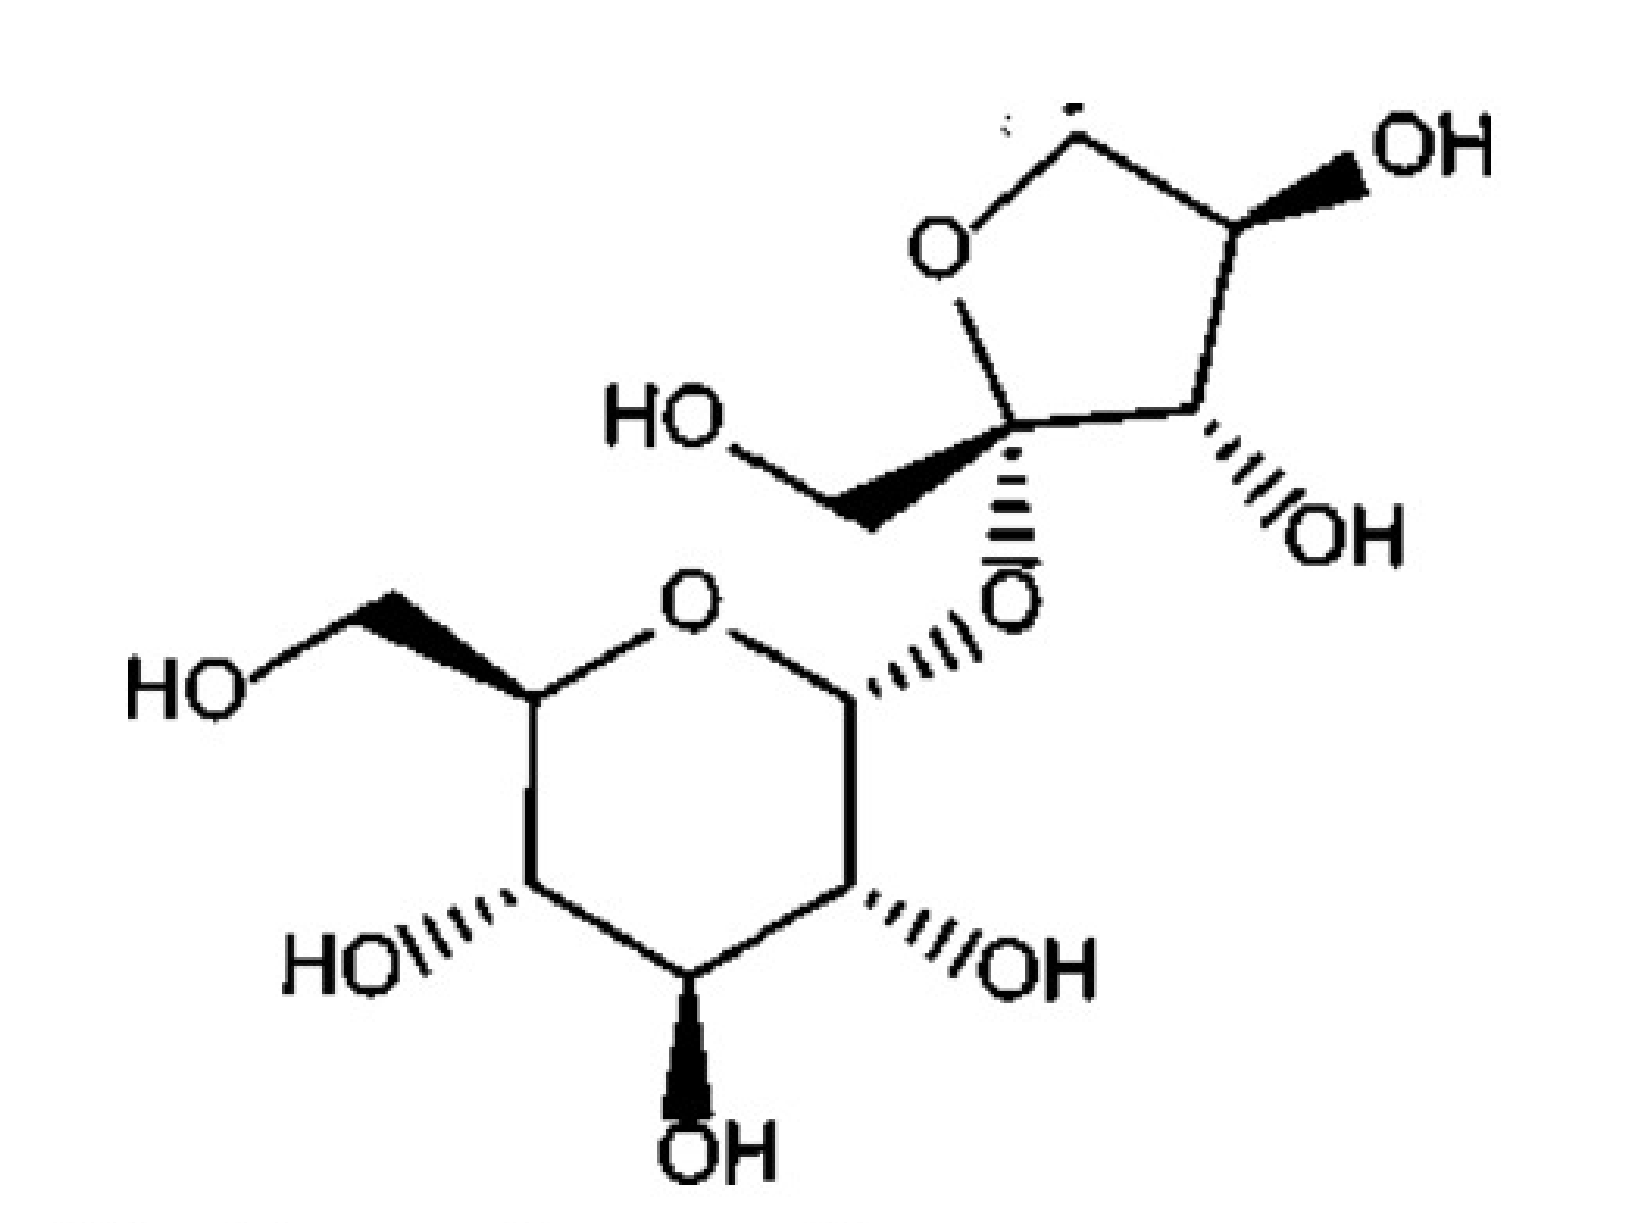
\includegraphics[width=0.45\textwidth]{images_crop_hoa11_de13/saccharose_structure.png}
\end{center}
Số nhóm chức alcohol trong một phân tử saccharose là bao nhiêu?
\choice
{3}
{5}
{\True 8}
{11}
\loigiai{
Phân tử saccharose (\ce{C12H22O11}) có 8 nhóm \ce{-OH} alcohol (gồm 3 nhóm \ce{-OH} bậc I và 5 nhóm \ce{-OH} bậc II).
}
\end{ex}

\Closesolutionfile{ans}

\bigskip
\noindent\textbf{\large PHẦN II. Câu trắc nghiệm đúng sai.}
\textit{Thí sinh trả lời từ câu 1 đến câu 4. Trong mỗi ý a), b), c), d) ở mỗi câu, thí sinh chọn đúng hoặc sai.}
\vspace{0.2cm}

% Câu 1 Phần II
\begin{ex}
Khái niệm và tính chất của dẫn xuất halogen.\\
Trong phòng thí nghiệm, học sinh quan sát thí nghiệm thuỷ phân ethyl bromide với dung dịch \ce{NaOH}.
\choiceTF
{\True Dẫn xuất halogen là hợp chất hữu cơ trong đó một hoặc nhiều nguyên tử hydrogen được thay thế bởi nguyên tử halogen}
{\True Ethyl bromide có thể tham gia phản ứng thế với \ce{NaOH} để tạo ra ethanol và \ce{NaBr}}
{Phản ứng giữa ethyl bromide và \ce{NaOH} tạo ra sản phẩm là \ce{NaCl} và nước}
{\True Từ kết quả thí nghiệm, có thể suy ra dẫn xuất halogen có khả năng tham gia phản ứng với \ce{OH^-} để tạo hợp chất chứa nhóm \ce{-OH}}
\loigiai{
- a) ĐÚNG: Định nghĩa chuẩn về dẫn xuất halogen.\\
- b) ĐÚNG, c) SAI: Phản ứng: \ce{C2H5Br + NaOH ->[t^\circ] C2H5OH + NaBr}.\\
- d) ĐÚNG: Nhóm \ce{-Br} được thay thế bằng nhóm \ce{-OH}.\\
$\Rightarrow$ a: ĐÚNG, b: ĐÚNG, c: SAI, d: ĐÚNG.
}
\end{ex}

% Câu 2 Phần II
\begin{ex}
Khái niệm và bậc của alcohol.\\
Trong phòng thí nghiệm, học sinh được giao nhiệm vụ nhận diện bậc của các alcohol thông qua công thức cấu tạo.
\choiceTF
{Alcohol là hợp chất hữu cơ chứa nhóm \ce{-OH} liên kết với nguyên tử carbon}
{\True Công thức tổng quát của alcohol no, đơn chức, mạch hở là \ce{C_nH_{2n+1}OH} ($n \ge 1$)}
{\True Alcohol bậc hai là alcohol trong đó nhóm \ce{-OH} liên kết với nguyên tử carbon bậc hai}
{\True Để phân biệt các bậc của alcohol, có thể sử dụng phương pháp xác định vị trí nhóm \ce{-OH} trong cấu trúc phân tử}
\loigiai{
- a) SAI: Nhóm \ce{-OH} phải liên kết trực tiếp với nguyên tử carbon no.\\
- b) ĐÚNG: Dãy đồng đẳng alcohol no, đơn chức, mạch hở.\\
- c) ĐÚNG: Bậc alcohol là bậc của C liên kết trực tiếp với nhóm \ce{-OH}.\\
- d) ĐÚNG: Xác định vị trí nhóm \ce{-OH} gắn vào C bậc mấy giúp phân loại bậc alcohol.\\
$\Rightarrow$ a: SAI, b: ĐÚNG, c: ĐÚNG, d: ĐÚNG.
}
\end{ex}

% Câu 3 Phần II
\begin{ex}
Tính chất vật lý của alcohol.\\
Trong thực tế, ethanol được sử dụng làm dung môi trong phòng thí nghiệm nhờ tính chất tan tốt trong nước.
\choiceTF
{\True Ethanol ở điều kiện thường tồn tại ở trạng thái lỏng}
{Nhiệt độ sôi của alcohol giảm khi số nguyên tử carbon trong mạch tăng}
{\True Alcohol có khả năng tan tốt trong nước nhờ liên kết hydrogen giữa nhóm \ce{-OH} và nước}
{Methanol có nhiệt độ sôi cao hơn ethanol do khối lượng phân tử nhỏ hơn}
\loigiai{
- a) ĐÚNG: Ethanol là chất lỏng không màu.\\
- b) SAI: Khi số C tăng, nhiệt độ sôi tăng dần.\\
- c) ĐÚNG: Liên kết hydrogen giúp các alcohol đầu dãy tan vô hạn trong nước.\\
- d) SAI: Methanol sôi ở $64{,}7^\circ\text{C}$, thấp hơn ethanol ($78{,}3^\circ\text{C}$).\\
$\Rightarrow$ a: ĐÚNG, b: SAI, c: ĐÚNG, d: SAI.
}
\end{ex}

% Câu 4 Phần II
\begin{ex}
Thí nghiệm phenol tác dụng với nước bromine.\\
Thực hiện thí nghiệm cho phenol phản ứng với nước bromine cho thấy khi nhỏ nước bromine vào dung dịch phenol, xuất hiện kết tủa trắng. Cho các mệnh đề sau:
\choiceTF
{\True Kết tủa trắng là 2,4,6-tribromophenol}
{\True Phản ứng thế bromine xảy ra ở vị trí \textit{ortho} và \textit{para} so với nhóm \ce{-OH}}
{\True Phản ứng này dùng để nhận biết phenol}
{\True Nguyên tử bromine thế vào vòng benzene làm mất màu nước bromine}
\loigiai{
Phenol tác dụng với nước bromine tạo kết tủa trắng 2,4,6-tribromophenol và làm mất màu dung dịch nước bromine:\\
\ce{C6H5OH + 3Br2 -> C6H2Br3OH v + 3HBr}.\\
Phản ứng thế vào cả 3 vị trí \textit{ortho} và \textit{para}, là phản ứng đặc trưng để nhận biết phenol.\\
$\Rightarrow$ Cả 4 ý a, b, c, d đều ĐÚNG.
}
\end{ex}

\bigskip
\noindent\textbf{\large PHẦN III. Câu trắc nghiệm yêu cầu trả lời ngắn.}
\textit{Thí sinh trả lời từ câu 1 đến câu 6.}
\vspace{0.2cm}

% Câu 1 Phần III
\begin{ex}
Cho công thức khung phân tử của dẫn xuất halogen X như hình dưới đây:
\begin{center}
	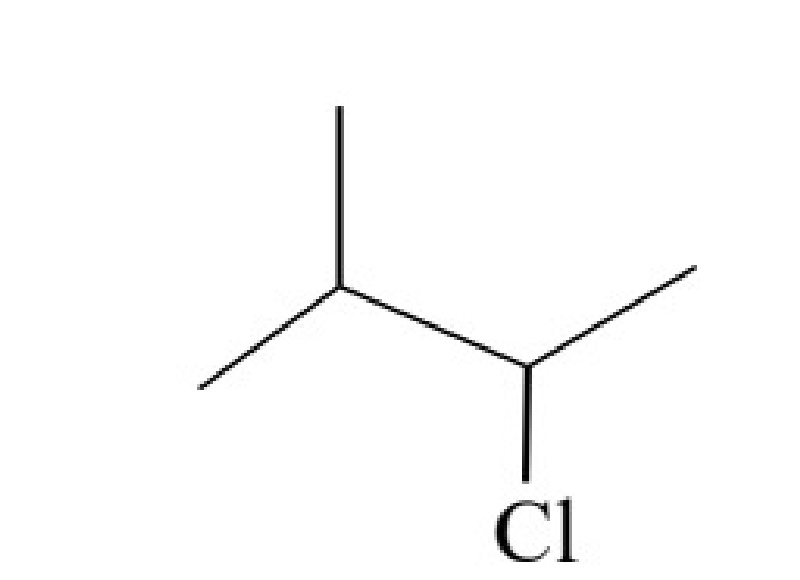
\includegraphics[width=0.25\textwidth]{images_crop_hoa11_de13/dan_xuat_halogen_x.png}
\end{center}
Số nguyên tử carbon có trong một phân tử chất X là bao nhiêu?
\shortans{5}
\loigiai{
Chất X là 2-chloro-3-methylbutane, có công thức cấu tạo \ce{(CH3)2CH-CH(Cl)-CH3}, công thức phân tử là \ce{C5H11Cl}. Số nguyên tử carbon trong phân tử là \textbf{5}.
}
\end{ex}

% Câu 2 Phần III
\begin{ex}
Fluoroethane (\ce{CH3CH2F}) từng được sử dụng làm chất làm lạnh, được tạo ra theo phản ứng:
\[
\ce{CH2=CH2 + HF -> CH3CH2F} \quad \Delta_r H^\circ_{298} = -73\text{ kJ}
\]
Dựa vào năng lượng liên kết $E_b$ (kJ/mol): C-H: 413; C=C: 614; H-F: 565; C-C: 347. Hãy xác định năng lượng liên kết C-F (kJ/mol) trong phân tử fluoroethane.
\shortans{492}
\loigiai{
Áp dụng công thức tính biến thiên enthalpy theo năng lượng liên kết:
\[
\Delta_r H^\circ_{298} = [E_b(\ce{C=C}) + 4E_b(\ce{C-H}) + E_b(\ce{H-F})] - [E_b(\ce{C-C}) + 5E_b(\ce{C-H}) + E_b(\ce{C-F})]
\]
\[
-73 = 614 + 565 - 347 - 413 - E_b(\ce{C-F})
\]
\[
-73 = 419 - E_b(\ce{C-F}) \implies E_b(\ce{C-F}) = 419 + 73 = 492\text{ kJ/mol}.
\]
$\Rightarrow$ Đáp số: \textbf{492}.
}
\end{ex}

% Câu 3 Phần III
\begin{ex}
Xylitol là một hợp chất hữu cơ được sử dụng làm chất tạo ngọt tự nhiên cho thực phẩm ăn kiêng và kẹo cao su, có công thức cấu tạo như hình dưới:
\begin{center}
	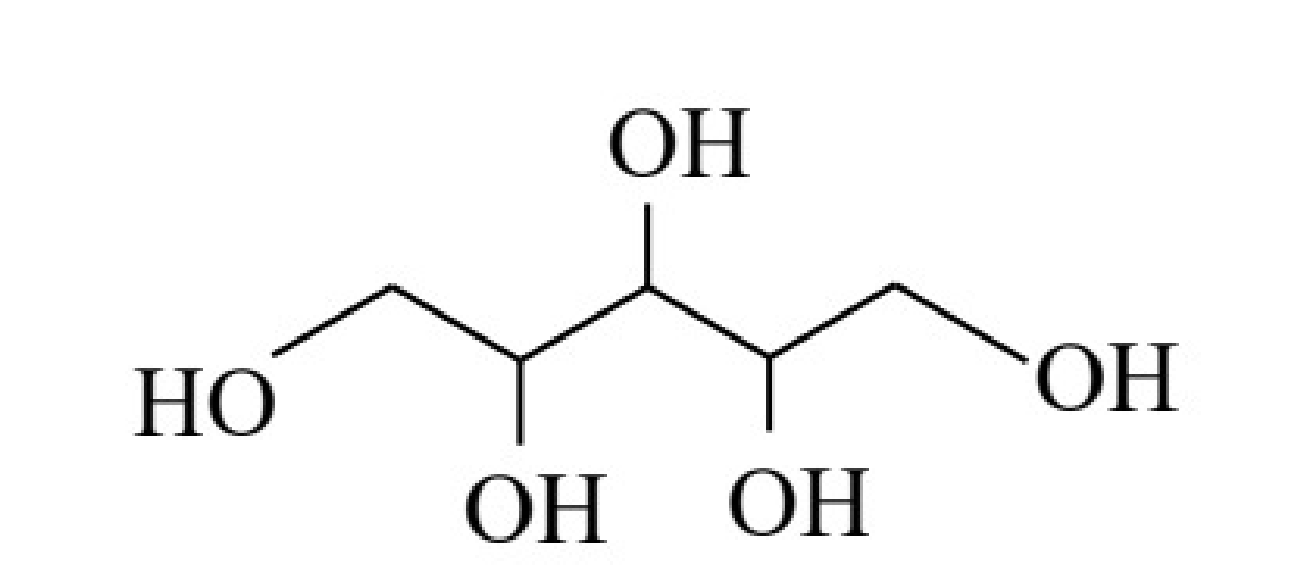
\includegraphics[width=0.38\textwidth]{images_crop_hoa11_de13/xylitol_structure.png}
\end{center}
Trong một phân tử Xylitol có bao nhiêu nhóm chức alcohol (\ce{-OH})?
\shortans{5}
\loigiai{
Công thức cấu tạo của Xylitol là \ce{HO-CH2-[CH(OH)]3-CH2-OH}. Phân tử chứa \textbf{5} nhóm chức alcohol (\ce{-OH}).
}
\end{ex}

% Câu 4 Phần III
\begin{ex}
Catechin là chất chống oxi hoá mạnh có trong lá chè tươi và nhiều loại hoa quả, có tác dụng phòng ngừa bệnh tim mạch và ung thư. Công thức cấu tạo của catechin được cho như hình dưới:
\begin{center}
	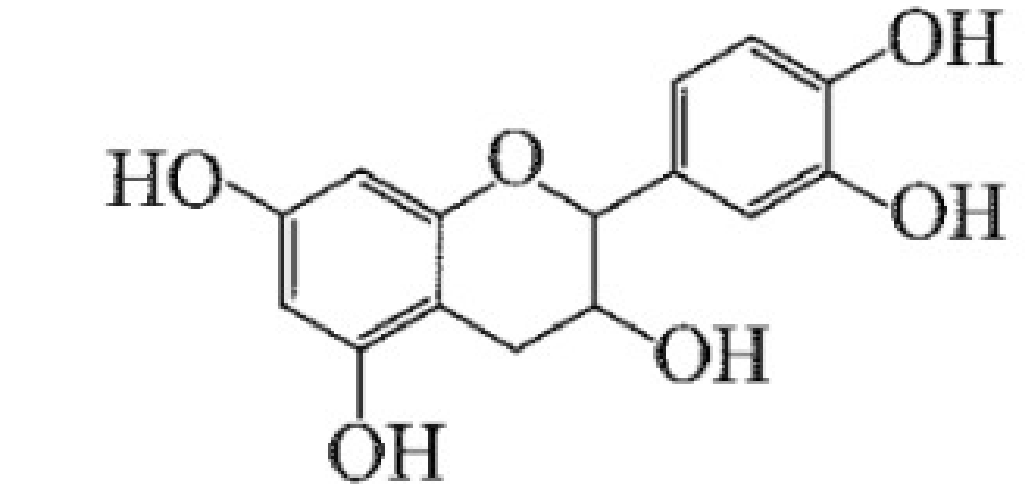
\includegraphics[width=0.42\textwidth]{images_crop_hoa11_de13/catechin_structure.png}
\end{center}
Số nguyên tử carbon có trong một phân tử catechin là bao nhiêu?
\shortans{15}
\loigiai{
Phân tử catechin có công thức phân tử là \ce{C15H14O6}, gồm 2 vòng benzene (mỗi vòng 6 carbon) và 1 vòng pyran 3 carbon $\implies 6 + 6 + 3 = 15$ nguyên tử carbon.
}
\end{ex}

% Câu 5 Phần III
\begin{ex}
Một mẫu hơi thở của người tham gia giao thông có thể tích 52,5 mL được thổi vào thiết bị Breathalyzer chứa 3 mL dung dịch \ce{K2Cr2O7} nồng độ 0,042 mg/mL trong môi trường acid \ce{H2SO4}. Toàn bộ \ce{C2H5OH} trong hơi thở bị oxi hóa hoàn toàn thành \ce{CH3COOH} theo phản ứng:
\[
\ce{3C2H5OH + 2K2Cr2O7 + 8H2SO4 -> 3CH3COOH + 2K2SO4 + 2Cr2(SO4)3 + 11H2O}
\]
Biết dung dịch chuyển hoàn toàn từ màu da cam sang màu xanh của \ce{Cr^{3+}}. Nồng độ alcohol trong hơi thở của người đó là bao nhiêu mg/L? (Làm tròn đến ba chữ số thập phân).
\shortans{0,563}
\loigiai{
- Khối lượng \ce{K2Cr2O7} phản ứng: $m = 3 \times 0{,}042 = 0{,}126\text{ mg} = 1{,}26 \times 10^{-4}\text{ g}$.\\
- Số mol \ce{K2Cr2O7}: $n = \dfrac{1{,}26 \times 10^{-4}}{294} \approx 4{,}2857 \times 10^{-7}\text{ mol}$.\\
- Số mol \ce{C2H5OH}: $n_{\text{cồn}} = 1{,}5 \times 4{,}2857 \times 10^{-7} \approx 6{,}4286 \times 10^{-7}\text{ mol}$.\\
- Khối lượng ethanol: $m_{\text{cồn}} = 6{,}4286 \times 10^{-7} \times 46 \approx 0{,}02957\text{ mg}$.\\
- Nồng độ trong 1 lít khí thở:
\[
C = \dfrac{0{,}02957\text{ mg}}{52{,}5\text{ mL}} \times 1000\text{ mL} \approx 0{,}563\text{ mg/L}.
\]
$\Rightarrow$ Đáp số: \textbf{0,563}.
}
\end{ex}

% Câu 6 Phần III
\begin{ex}
Từ $m\text{ kg}$ gạo (chứa 75\% khối lượng tinh bột) thực hiện quá trình lên men ethyl alcohol với hiệu suất chung 80\%, thu được 10 lít ethyl alcohol 46$^\circ$. Biết khối lượng riêng của ethyl alcohol là 0,8 g/mL. Giá trị của $m$ là bao nhiêu kg? (Làm tròn đến một chữ số thập phân).
\shortans{10,8}
\loigiai{
- Thể tích ethyl alcohol nguyên chất: $V = 10 \times 46\% = 4{,}6\text{ lít} = 4600\text{ mL}$.\\
- Khối lượng ethanol: $m = 4600 \times 0{,}8 = 3680\text{ g} = 3{,}68\text{ kg}$.\\
- Quá trình lên men:\\
\ce{(C6H10O5)_n -> n C6H12O6 -> 2n C2H5OH}\\
162 kg tinh bột $\longrightarrow$ 92 kg ethanol.\\
Khối lượng tinh bột theo lý thuyết: $m_{\text{tb, lt}} = 3{,}68 \times \dfrac{162}{92} = 6{,}48\text{ kg}$.\\
- Do $H = 80\%$ và tinh bột chiếm 75\% gạo:
\[
m_{\text{gạo}} = \dfrac{6{,}48}{0{,}80 \times 0{,}75} = \dfrac{6{,}48}{0{,}60} = 10{,}8\text{ kg}.
\]
$\Rightarrow$ Đáp số: \textbf{10,8}.
}
\end{ex}

\bigskip
\noindent\textbf{\large PHẦN IV. Câu hỏi tự luận.}
\textit{Thí sinh trình bày lời giải chi tiết vào giấy làm bài.}
\vspace{0.2cm}

% Câu 1 Tự luận
\begin{ex}
Methyl tert-butyl ether (MTBE) có công thức cấu tạo \ce{CH3-O-C(CH3)3}, là phụ gia pha vào xăng nhằm làm tăng chỉ số octane của xăng dầu.\\
a) Viết phương trình hóa học của phản ứng tạo ra MTBE từ hai alcohol tương ứng. Vì sao phương pháp điều chế MTBE từ hai alcohol tương ứng không phù hợp để tổng hợp MTBE trong công nghiệp?\\
b) Trong công nghiệp, MTBE được sản xuất bằng phản ứng cộng methanol vào 2-methylpropene. Viết phương trình hóa học của phản ứng.

\loigiai{
a) Phương trình phản ứng điều chế MTBE từ hai alcohol tương ứng:
\[
\ce{CH3OH + (CH3)3C-OH ->[H2SO4 \text{ đặc},\, t^\circ] CH3-O-C(CH3)3 + H2O}
\]
Phương pháp này không phù hợp trong công nghiệp vì xảy ra sự tạo thành hỗn hợp 3 ether khác nhau (\ce{CH3OCH3}, MTBE, và di-tert-butyl ether) đồng thời tert-butyl alcohol rất dễ bị tách nước nội phân tử tạo alkene (2-methylpropene), dẫn đến hiệu suất thấp và tách tinh chế khó khăn.\\
b) Phương trình tổng hợp MTBE trong công nghiệp từ methanol và 2-methylpropene (xúc tác acid):
\[
\ce{CH3OH + CH2=C(CH3)2 ->[H^+,\, t^\circ] CH3-O-C(CH3)3}
\]
}

\end{ex}

% Câu 2 Tự luận
\begin{ex}
(SBT-KNTT) Một đèn cồn thí nghiệm chứa 100 mL cồn 90$^\circ$. Tính nhiệt lượng đèn cồn tỏa ra khi đốt cháy hết lượng cồn trên, biết khối lượng riêng của ethanol là 0,789 g/mL và nhiệt sinh ra khi đốt cháy 1 mol ethanol là 1 371 kJ/mol. (Làm tròn đến một chữ số thập phân).

\loigiai{
- Thể tích ethanol nguyên chất trong 100 mL cồn 90$^\circ$: $V = 100 \times 90\% = 90\text{ mL}$.\\
- Khối lượng ethanol: $m = 90 \times 0{,}789 = 71{,}01\text{ g}$.\\
- Số mol ethanol: $n = \dfrac{71{,}01}{46} \approx 1{,}5437\text{ mol}$.\\
- Lượng nhiệt toả ra khi đốt cháy hoàn toàn:
\[
Q = 1{,}5437 \times 1371 \approx 2116{,}4\text{ kJ}.
\]
\textbf{Kết luận:} Đèn cồn toả ra khoảng \textbf{2 116,4 kJ} nhiệt lượng.
}

\end{ex}

\newpage
\noindent\textbf{\large BẢNG ĐÁP ÁN THAM KHẢO PHẦN I}
\vspace{0.2cm}

\begin{center}
\begin{tabular}{|c|c|c|c|c|c|c|c|c|}
\hline
\textbf{1. C} & \textbf{2. C} & \textbf{3. B} & \textbf{4. C} & \textbf{5. C} & \textbf{6. A} & \textbf{7. A} & \textbf{8. A} & \textbf{9. B} \\
\hline
\textbf{10. A} & \textbf{11. C} & \textbf{12. A} & \textbf{13. D} & \textbf{14. C} & \textbf{15. B} & \textbf{16. C} & \textbf{17. C} & \textbf{18. C} \\
\hline
\end{tabular}
\end{center}

\bigskip
\noindent\textbf{\large BẢNG ĐÁP ÁN THAM KHẢO PHẦN II}
\vspace{0.2cm}

\begin{center}
\begin{tabular}{|c|c|c|c|c|}
\hline
\textbf{Câu} & \textbf{Ý a)} & \textbf{Ý b)} & \textbf{Ý c)} & \textbf{Ý d)} \\
\hline
\textbf{Câu 1} & Đ & Đ & S & Đ \\
\hline
\textbf{Câu 2} & S & Đ & Đ & Đ \\
\hline
\textbf{Câu 3} & Đ & S & Đ & S \\
\hline
\textbf{Câu 4} & Đ & Đ & Đ & Đ \\
\hline
\end{tabular}
\end{center}

\bigskip
\noindent\textbf{\large BẢNG ĐÁP ÁN THAM KHẢO PHẦN III}
\vspace{0.2cm}

\begin{center}
\begin{tabular}{|c|c|c|c|c|c|}
\hline
\textbf{Câu 1} & \textbf{Câu 2} & \textbf{Câu 3} & \textbf{Câu 4} & \textbf{Câu 5} & \textbf{Câu 6} \\
\hline
5 & 492 & 5 & 15 & 0{,}563 & 10{,}8 \\
\hline
\end{tabular}
\end{center}

\begin{center}
\textbf{--------- HẾT ---------}
\end{center}

\end{document}
